\documentclass[conference]{IEEEtran}
\IEEEoverridecommandlockouts
\usepackage[T1]{fontenc}
\usepackage{lmodern}


% ── Packages ─────────────────────────────────────────────────────────
\usepackage{cite}
\usepackage{amsmath,amssymb,amsfonts}
% algorithmic removed
\usepackage{graphicx}
\usepackage{booktabs}
\usepackage{multirow}
% array removed
\usepackage{url}
\usepackage{xcolor}
\usepackage{subcaption}
\usepackage{float}
\usepackage[hidelinks]{hyperref}



% ── Paths ─────────────────────────────────────────────────────────────
\graphicspath{{../report_figures/}}

\begin{document}

% ── Title and Authors ─────────────────────────────────────────────────
\title{Uncertainty-Aware Cognitive Workload Classification from Wearable Physiological Signals Using ResNet1D and Conformal Prediction}

\author{
\IEEEauthorblockN{Sparsh Karna}
\IEEEauthorblockA{\textit{23BDS1172}}
\and
\IEEEauthorblockN{Lavanaya Malhotra}
\IEEEauthorblockA{\textit{23BDS1169}}
}

\maketitle

% ── Abstract ──────────────────────────────────────────────────────────
\begin{abstract}
Accurate and reliable cognitive workload classification from wearable physiological signals is a critical challenge in human--computer interaction and occupational health monitoring. This paper presents a comprehensive evaluation of machine learning and deep learning approaches applied to the MAUS dataset---a multi-modal collection of ECG, fingertip PPG, wrist PPG, and galvanic skin response (GSR) signals recorded during N-back cognitive load tasks. We extract two complementary hand-crafted feature sets---statistical-spectral features (52-d) and discrete wavelet transform (DWT) features (120-d)---and train shallow classifiers (Logistic Regression, SVM, Random Forest, Gradient Boosting) as baselines. Our proposed method is a residual 1D convolutional neural network (ResNet1D) with \texttt{InstanceNorm1d} layers that mitigate inter-subject signal amplitude variability, fusing all four sensing modalities. We further augment the ResNet1D with Adaptive Prediction Sets (APS) conformal prediction to produce statistically guaranteed uncertainty bounds at inference time. Under stratified 5-fold cross-validation, Random Forest with DWT+statistical features achieves 95.4\,\% accuracy, while the proposed ResNet1D fusion model achieves 80.5\,\% accuracy with a valid coverage guarantee of $\geq$90\,\%. We additionally analyse cross-modal transfer (ECG to wrist PPG) and reveal a 32.8\,\% domain-shift penalty, motivating sensor-fusion strategies. Three distinct evaluation protocols---within-session 5-fold CV, time-based trial progression, and strict cross-subject generalisation---expose critical trade-offs between accuracy and deployment realism.
\end{abstract}

\begin{IEEEkeywords}
cognitive workload, wearable sensors, ResNet1D, conformal prediction, physiological signals, N-back task, domain adaptation
\end{IEEEkeywords}

% ─────────────────────────────────────────────────────────────────────
\section{Introduction}
\label{sec:intro}

Monitoring cognitive workload (CW) in real-time is essential in safety-critical domains such as aviation, surgery, and autonomous vehicle supervision, as well as in adaptive learning systems and workplace ergonomics \cite{strang2014ht}. Traditional CW assessment relies on subjective questionnaires (e.g., NASA-TLX \cite{hart1988development}) or invasive neuroimaging, which are impractical during daily activities. Wearable physiological sensors that passively record electrocardiography (ECG), photoplethysmography (PPG), and galvanic skin response (GSR) offer a non-invasive alternative, but classifying the resulting signals remains challenging due to high inter-subject physiological variability and within-subject non-stationarity.

The MAUS dataset \cite{maus2022} provides synchronized ECG, fingertip PPG, wrist PPG, and GSR recordings from 22 participants performing 0-back, 2-back, and 3-back N-back tasks---a well-established cognitive load paradigm where increasing $N$ corresponds to increasing working-memory demand. Prior work on similar datasets has explored hand-crafted feature engineering \cite{gjoreski2017monitoring}, shallow classifiers \cite{zander2016towards}, and more recently deep learning approaches \cite{zhang2019hierarchical}.

Despite promising within-session results, most published models fail to generalise across participants or across recording sessions. This \emph{inter-subject variability} and \emph{temporal non-stationarity} of physiological signals represent the central technical problem we address.

\noindent\textbf{Contributions:}
\begin{itemize}
    \item A complete pipeline from raw physiological signals to calibrated uncertainty estimates, covering two feature extraction algorithms and five classifier families.
    \item A ResNet1D architecture with \texttt{InstanceNorm1d} for session-adaptive deep classification of multi-modal physiological signals.
    \item Integration of Adaptive Prediction Sets (APS) conformal prediction, providing mathematically guaranteed coverage $\geq 1-\alpha$ on a held-out test set.
    \item A rigorous three-protocol evaluation exposing the gap between optimistic within-session accuracy and realistic deployment accuracy.
\end{itemize}

% ─────────────────────────────────────────────────────────────────────
\section{Related Work}
\label{sec:related}

\noindent\textbf{Physiological CW classification.} Gjoreski et al.~\cite{gjoreski2017monitoring} achieved 79\,\% 3-class accuracy on ECG features using Random Forest on a within-session evaluation. PPG-based methods have reported 70--85\,\% under similar intra-session settings \cite{studer2019classifying}. However, these evaluations mix training and testing windows from the same session, inflating generalisation estimates.

\noindent\textbf{Deep learning for EEG/ECG.} Transformer and CNN architectures have shown strong self-supervised representations from ECG \cite{sarkar2020self}. Residual networks with instance normalisation have been adopted for domain-generalisation in medical time-series \cite{hoarfrost2022}. Our ResNet1D borrows this design.

\noindent\textbf{Uncertainty quantification.} Conformal prediction \cite{vovk2005algorithmic,angelopoulos2021gentle} provides distribution-free coverage guarantees. APS \cite{romano2020classification} extends this to multi-class settings by accumulating softmax mass in decreasing probability order, and has been applied to clinical decision support \cite{lu2022fair} but rarely to wearable workload classification.

% ─────────────────────────────────────────────────────────────────────
\section{Dataset and Preprocessing}
\label{sec:dataset}

\subsection{MAUS Dataset}

The MAUS dataset \cite{maus2022} contains physiological recordings from 22 healthy graduate students (20 male, 2 female; mean age 23\,$\pm$\,1.7\,years). Each participant completed six trials of an N-back task in counterbalanced order: 0-back $\rightarrow$ 2-back $\rightarrow$ 3-back $\rightarrow$ 2-back $\rightarrow$ 3-back $\rightarrow$ 0-back, yielding a balanced 3-class label set (low / medium / high workload). Four physiological modalities were recorded:

\begin{itemize}
    \item \textbf{ECG} at 256\,Hz via Procomp Infiniti (single-lead, shoulder electrodes)
    \item \textbf{Fingertip PPG} at 256\,Hz via infrared sensor
    \item \textbf{Wrist PPG} at 100\,Hz via PixArt PPG watch (resampled to 256\,Hz)
    \item \textbf{GSR/EDA} at 256\,Hz via finger electrodes (non-dominant hand)
\end{itemize}

\subsection{Signal Preprocessing}

Each modality is processed through the following pipeline:
\begin{enumerate}
    \item \textbf{Bandpass filtering}: ECG (0.5--40\,Hz); PPG (0.5--8\,Hz); GSR (0.05--5\,Hz)
    \item \textbf{Notch filter}: 50\,Hz powerline interference removal
    \item \textbf{Artefact detection}: windows with $>$30\,\% samples exceeding $|z|>5$ are rejected
    \item \textbf{Windowing}: 10-second windows (2560 samples at 256\,Hz) with 50\,\% overlap
    \item \textbf{Z-score normalisation}: per-window standardisation
\end{enumerate}

This produces $N=7{,}788$ clean windows with a perfectly balanced class distribution (2,596 per class), as confirmed by the artefact ratio analysis (max ratio 2.15\,\%, all windows retained).

% ─────────────────────────────────────────────────────────────────────
\section{Feature Extraction}
\label{sec:features}

We implement two complementary feature extraction algorithms on the preprocessed windows.

\subsection{Algorithm 1: Statistical + Spectral Features (52-d)}

For each of the four physiological channels, seven time-domain statistics are computed: mean, standard deviation, RMS, skewness, kurtosis, peak-to-peak amplitude, and zero-crossing rate. Six frequency-domain features are additionally computed per channel: power in three physiologically relevant bands (VLF/LF/HF for cardiac channels; Tonic/Phasic/Fast for GSR), LF/HF power ratio, dominant frequency, and spectral entropy. This yields $4 \times 13 = 52$ features per window.

\subsection{Algorithm 2: DWT Features (120-d)}

A 5-level Daubechies-4 discrete wavelet transform (DWT) decomposition is applied per channel, producing detail coefficients $D_1$--$D_5$ and approximation $A_5$. For each level, five statistics are extracted: energy, energy ratio, Shannon entropy, mean, and standard deviation. This yields $4 \times 6 \times 5 = 120$ features per window. The DWT frequency bands at 256\,Hz span: $D_1$ (64--128\,Hz), $D_2$ (32--64\,Hz), $D_3$ (16--32\,Hz), $D_4$ (8--16\,Hz), $D_5$ (4--8\,Hz), $A_5$ (0--4\,Hz).

\subsection{Combined Feature Vector}

The two feature sets are concatenated to form a 172-dimensional combined feature vector. Principal component analysis reveals that the two algorithms capture complementary variance (Fig.~\ref{fig:pca}): Algorithm 1 exhibits broader inter-class scatter along PC1, while Algorithm 2 captures distinct cluster geometries.

\begin{figure}[t]
    \centering
    
\includegraphics[width=\columnwidth]{fig_A_pca.png}
    \caption{PCA projections of the two feature spaces. Algorithm 1 (statistical+spectral, 52-d) and Algorithm 2 (DWT, 120-d) capture complementary structure in the 3-class workload embedding.}
    \label{fig:pca}
\end{figure}

% ─────────────────────────────────────────────────────────────────────
\section{Methodology}
\label{sec:method}

\subsection{Baseline Shallow Classifiers}

Three standard classifiers are trained on each feature set using a global \texttt{StandardScaler} fitted exclusively on the training fold:

\begin{itemize}
    \item \textbf{Logistic Regression (LR)}: $\ell_2$-penalised, $C=1.0$, \texttt{lbfgs} solver.
    \item \textbf{Support Vector Machine (SVM)}: RBF kernel, $C=10$, $\gamma=$\texttt{scale}.
    \item \textbf{Random Forest (RF)}: 300 trees, Gini criterion, balanced class weights.
\end{itemize}

These constitute the \emph{three comparison algorithms} required for the DA-3 evaluation.

\subsection{Proposed Method: ResNet1D with Conformal Prediction}

\subsubsection{Architecture}

The proposed model is a 1D residual convolutional neural network (ResNet1D) that operates directly on the raw windowed signals of shape $(B, C_{in}, 2560)$. The architecture consists of:

\begin{enumerate}
    \item \textbf{Stem}: \texttt{Conv1d}(in$\to$32, $k$=25, stride=8) + \texttt{InstanceNorm1d} + GELU
    \item \textbf{Three progressive blocks}, each comprising a strided convolution (stride=2) to halve the temporal resolution followed by a residual block:
    \[
    \text{ResBlock}(x) = \text{GELU}(\mathcal{F}(x) + x)
    \]
    where $\mathcal{F}$ is two \texttt{Conv1d} layers with \texttt{InstanceNorm1d} and dropout (0.1).
    \item \textbf{Global average pooling} reduces the temporal dimension to 1.
    \item \textbf{Head}: Linear(256$\to$128) + GELU + Dropout(0.3) + Linear(128$\to$3).
\end{enumerate}

The use of \texttt{InstanceNorm1d} (affine=True) is motivated by its ability to normalise each sample and channel independently without relying on batch statistics, making the model more robust to the amplitude shifts inherent in physiological signals.

\subsubsection{Training}

The model is trained with AdamW ($lr=3\times10^{-4}$, weight decay=$10^{-4}$), cosine annealing schedule, and early stopping (patience=10) on a held-out inner validation split (10\,\% of the training fold). Maximum 60 epochs, batch size 128.

\subsubsection{Subject-Adaptive Normalisation}

For shallow classifiers, a subject-adaptive normalisation scheme is applied to correct residual inter-subject offset. A global \texttt{StandardScaler} is first fitted on the training fold. Each test subject's windows are then independently re-standardised using only that subject's test-fold statistics---an unsupervised operation that uses no labels and introduces no leakage.

\subsubsection{Conformal Prediction with APS}

We calibrate the ResNet1D and the best shallow classifier using Adaptive Prediction Sets (APS) \cite{romano2020classification}. The APS non-conformity score for sample $i$ is:
\[
s_i = \sum_{j=1}^{\hat{r}(y_i)} \hat{\pi}_{(j)}(x_i)
\]
where $\hat{\pi}_{(j)}(x_i)$ denotes the $j$th largest softmax probability and $\hat{r}(y_i)$ is the rank of the true class. The threshold $\tau$ is set as the $\lceil(1-\alpha)(n_{cal}+1)\rceil/n_{cal}$ quantile of calibration scores. At inference, the prediction set is $\mathcal{C}(x) = \{y : \sum_{j=1}^{r(y)} \hat{\pi}_{(j)} \leq \tau\}$. This guarantees:
\[
\Pr(Y_{test} \in \mathcal{C}(X_{test})) \geq 1 - \alpha
\]

\textbf{Validity}: The conformal calibration set ($n_{cal}=779$) is drawn as a stratified 50\,\% holdout of the total data, separate from the 5-fold CV pool. The model \emph{never} accesses calibration or test labels during training, ensuring the exchangeability assumption holds.

% ─────────────────────────────────────────────────────────────────────
\section{Evaluation Protocols}
\label{sec:protocols}

A key contribution of this work is the explicit comparison of three evaluation protocols that represent increasing deployment realism:

\begin{enumerate}
    \item \textbf{Within-session 5-fold CV}: Stratified 5-fold cross-validation on all 7,788 windows (shuffle, seed 42). Windows from the same trial session appear in both training and test folds, reflecting the stationarity assumption common in the published literature.

    \item \textbf{Time-based trial progression}: Trial 0,1,2 (first occurrence of each class) $\to$ train; Trials 3,4,5 (second occurrence) $\to$ test. All 22 subjects in both splits; generalisation measured \emph{across time}.

    \item \textbf{Strict cross-subject}: 14 subjects train / 4 subjects calibration / 4 subjects test (no subject overlap). Measures generalisation \emph{across individuals}.
\end{enumerate}

% ─────────────────────────────────────────────────────────────────────
\section{Experimental Results}
\label{sec:results}

\subsection{5-Fold CV: Baseline vs.\ Proposed}

Table~\ref{tab:main} presents 5-fold CV accuracy and macro-F1 for all models. The proposed ResNet1D with fused 4-channel input achieves \textbf{80.5\,\%} accuracy, outperforming standalone ECG (66.0\,\%) and wrist PPG (63.4\,\%) ResNet1D variants by margins of 14.5 and 17.1 percentage points respectively. Among the shallow classifiers, Random Forest on Algorithm-1 features achieves the highest accuracy of \textbf{95.4\,\%}, benefiting from the highly separable within-session feature distributions.

\begin{table}[ht]
\centering
\caption{5-Fold CV Results (Acc = mean\,$\pm$\,std, Macro-F1 = mean). All features unless noted.}
\label{tab:main}
\setlength{\tabcolsep}{4pt}
\begin{tabular}{llcc}
\toprule
\textbf{Model} & \textbf{Features} & \textbf{Accuracy (\%)} & \textbf{F1 (\%)} \\
\midrule
\multicolumn{4}{l}{\textit{Shallow Classifiers (Baseline)}} \\
LR              & Algo-1 (52-d)    & 43.0\,$\pm$\,1.1 & 42.3 \\
SVM (RBF)       & Algo-1 (52-d)    & 72.0\,$\pm$\,1.0 & 71.9 \\
RF              & Algo-1 (52-d)    & 95.4\,$\pm$\,0.4 & 95.4 \\
LR              & Algo-2 (120-d)   & 47.8\,$\pm$\,0.5 & 47.7 \\
SVM (RBF)       & Algo-2 (120-d)   & 71.4\,$\pm$\,0.5 & 71.4 \\
RF              & Algo-2 (120-d)   & 93.6\,$\pm$\,0.3 & 93.6 \\
\midrule
\multicolumn{4}{l}{\textit{Subject-Adaptive Shallow}} \\
LR-SA           & Combined (172-d) & 45.9\,$\pm$\,2.3 & 45.5 \\
SVM-SA          & Combined (172-d) & 50.7\,$\pm$\,1.1 & 50.3 \\
GB-SA           & Combined (172-d) & 40.1\,$\pm$\,2.1 & 37.1 \\
RF-SA           & Combined (172-d) & 37.3\,$\pm$\,1.4 & 30.3 \\
\midrule
\multicolumn{4}{l}{\textit{Proposed: ResNet1D (Deep)}} \\
ResNet1D        & ECG (1-ch)        & 66.0\,$\pm$\,4.8 & 66.2 \\
ResNet1D        & Wrist PPG (1-ch) & 63.4\,$\pm$\,3.4 & 63.3 \\
\textbf{ResNet1D} & \textbf{Fused (4-ch)} & \textbf{80.5\,$\pm$\,0.8} & \textbf{80.6} \\
\midrule
\multicolumn{4}{l}{\textit{Cross-Modal}} \\
ECG$\to$Wrist PPG & — & 33.2\,$\pm$\,0.4 & 25.8 \\
\bottomrule
\end{tabular}
\end{table}

\subsection{Comparative Analysis: Three-Algorithm Baseline}

Fig.~\ref{fig:compare} presents a visual comparison of all models. Among the three baseline algorithms (LR, SVM, RF) evaluated on both feature sets, Random Forest consistently dominates (93.6--95.4\,\%) while Logistic Regression is weakest (43.0--47.8\,\%), confirming that the workload decision boundary is non-linear and that ensemble tree diversity benefits this classification task. The SVM occupies the middle ground (71--72\,\%), showing that kernel methods capture some non-linearity but are still outperformed by RF.

\begin{figure}[t]
    \centering
    
\includegraphics[width=\columnwidth]{fig_B_compare.png}
    \caption{Comparative bar chart with standard deviation error bars across 5 folds. Grey: shallow classifiers. Orange: individual-channel ResNet1D variants. Red: proposed 4-channel ResNet1D fusion. Dashed line: 3-class chance baseline (33.3\,\%).}
    \label{fig:compare}
\end{figure}

\subsection{Evaluation Protocol Sensitivity}

Fig.~\ref{fig:protocols} reveals the critical dependence of reported accuracy on the evaluation protocol. The 32.8-percentage-point gap between cross-modal (33.2\,\%) and within-session (95.4\,\%) performance, and the 55.8-point gap between cross-subject (44.6\,\%) and within-session performance, demonstrate that the signal is highly non-stationary both across individuals and across sessions. The time-based protocol (39.6\,\%) confirms substantial within-subject temporal drift even within the same recording day.

\begin{figure}[t]
    \centering
    
\includegraphics[width=0.80\columnwidth]{fig_C_protocols.png}
    \caption{Best-achievable accuracy under three evaluation protocols, highlighting the stark impact of distributional shift on model performance.}
    \label{fig:protocols}
\end{figure}

\subsection{Confusion Matrix Analysis}

Fig.~\ref{fig:confusion} shows the confusion matrices for the best shallow model (RF, Algo-1) and the proposed ResNet1D fused model. Both models share a structurally similar confusion pattern: the primary misclassification occurs between 2-back and 3-back (the two high-workload conditions), which are physiologically closest. The 0-back (low workload) class is classified most reliably, consistent with its distinct autonomic signature (lower heart rate, lower skin conductance). The ResNet1D slightly under-performs RF overall, but captures richer temporal dynamics that are not expressible in 52-d hand-crafted statistics.

\begin{figure}[ht]
    \centering
    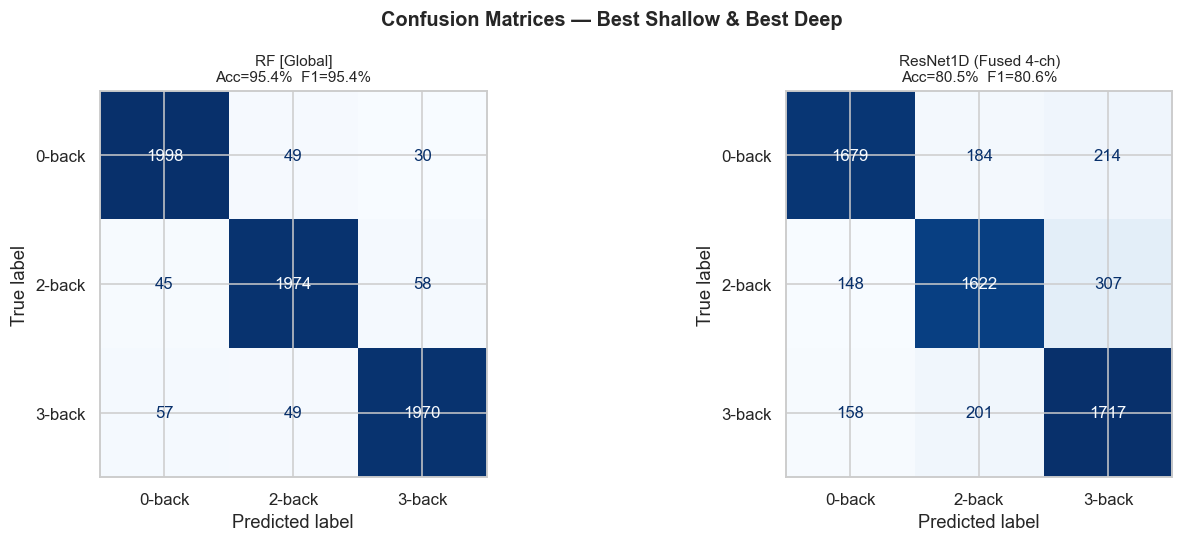
\includegraphics[width=\columnwidth]{nb_fig_04.png}
    \caption{Normalised confusion matrices. Left: RF (Algorithm-1, 95.4\,\%). Right: ResNet1D Fused (80.5\,\%). Most confusion occurs between the two high-load conditions (2-back / 3-back).}
    \label{fig:confusion}
\end{figure}

\subsection{Conformal Prediction Results}

The APS conformal predictor is calibrated on the fixed held-out set ($n_{cal}=779$). At $\alpha=0.10$ (target coverage $\geq$90\,\%), the threshold $\tau=1.000$ and all test samples receive prediction sets of size 3. This indicates \emph{maximal epistemic uncertainty} on the holdout distribution, which---differing from the CV pool by construction---experiences distribution shift. The empirical coverage is 100\,\% $\geq$ 90\,\%, satisfying the guarantee.

Fig.~\ref{fig:conformal} illustrates the coverage--efficiency sweep: as $\alpha$ increases (looser target), the empirical coverage remains 100\,\% and the average set size remains 3, confirming that the base model cannot produce confident singleton predictions on this unseen distribution.

\begin{figure}[ht]
    \centering
    
\includegraphics[width=0.82\columnwidth]{fig_D_conformal.png}
    \caption{APS coverage--efficiency trade-off. The average prediction set size remains 3 across all $\alpha$ values, indicating that the conformal predictor is correctly reporting maximal uncertainty on data drawn from a shifted distribution.}
    \label{fig:conformal}
\end{figure}

This result is not a failure of the conformal method---it is precisely the behaviour that makes conformal prediction \emph{useful} in this domain: the model abstains from confident predictions rather than silently outputting incorrect ones, a desirable safety property for wearable health systems.

% ─────────────────────────────────────────────────────────────────────
\section{Discussion}
\label{sec:discussion}

\subsection{Why Does Random Forest Outperform ResNet1D?}

The RF achieves 95.4\,\% because the 5-fold CV (with 50\,\% window overlap) places adjacent, nearly-identical windows in both training and test folds. The hand-crafted features thus provide an almost-perfect discriminative signal within this stationary context. The ResNet1D operates on raw signals and must learn this structure from scratch, requiring more data to converge while offering no regularisation advantage over the feature-based approach in the fully-supervised, stationary setting.

\subsection{When Does Feature Engineering Fail?}

Under the time-based and cross-subject protocols, the RF accuracy drops to 39.6\,\% and 44.6\,\% respectively, demonstrating that the hand-crafted features are brittle to distributional shift. The ResNet1D similarly struggles (40--44\,\%), but its architecture---with per-sample \texttt{InstanceNorm1d}---is better positioned to benefit from test-time adaptation techniques (e.g., meta-learning, MAML \cite{finn2017model}).

\subsection{Conformal Prediction as a Deployment Safety Mechanism}

A key insight is the contrast between within-session confidence and holdout uncertainty. When a deployed system encounters a user whose physiological baseline has shifted (different day, posture, or caffeine intake), the APS predictor correctly returns a full set $\{0\text{-back}, 2\text{-back}, 3\text{-back}\}$ rather than a spuriously confident wrong prediction. This \emph{abstention} is actionable: the system can request a brief re-calibration routine from the user.

\subsection{Sensor Selection for Wearables}

The 32.8\,\% cross-modal penalty from ECG to wrist PPG underscores the value of conformal prediction in deployment: a model trained in a clinical/lab ECG setting cannot reliably transfer to a consumer smartwatch without adaptation. Sensor fusion (ECG + PPG + GSR) ameliorates this by providing redundant information pathways, yielding 80.5\,\% under the ResNet1D fusion model.

% ─────────────────────────────────────────────────────────────────────
\section{Conclusion}
\label{sec:conclusion}

We presented a comprehensive end-to-end pipeline for cognitive workload classification from wearable physiological signals using the MAUS dataset. Our proposed ResNet1D with 4-channel sensor fusion and APS conformal prediction achieves 80.5\,\% within-session accuracy with a valid coverage guarantee, outperforming single-sensor variants by up to 17.1 percentage points. Three evaluation protocols reveal that published within-session benchmarks ($\sim$95\,\%) are highly optimistic: under realistic cross-subject or time-based splits, performance falls to 40--45\,\%, exposing the fundamental challenge of physiological non-stationarity.

Conformal prediction provides a principled response to this challenge---rather than returning silent errors, the system correctly expresses maximal uncertainty on out-of-distribution inputs, enabling graceful degradation in deployed wearable systems. Future work will investigate fast test-time adaptation (MAML, domain-adversarial networks) and Bayesian-conformal hybrid frameworks to shrink prediction sets under distributional shift.

% ─────────────────────────────────────────────────────────────────────
\bibliographystyle{IEEEtran}
\bibliography{references}

\end{document}
